%% =====================================================================
%%  Hito 2 - IMT-342 Robotica
%%  Grupo VEVAS
%%  Universidad Catolica Boliviana "San Pablo", Sede Tarija
%%  Departamento de Ciencias de la Tecnologia e Innovacion
%%  Carrera de Ingenieria Mecatronica
%%
%%  COMPILACION
%%  Clase IEEEtran, como exige la plantilla oficial del docente
%%  (hito_2_ieee_template.tex). IEEEtran viene instalada en Overleaf.
%%
%%      Overleaf:  subir la carpeta entera, compilar con pdfLaTeX, 2 veces.
%%      Local:     sudo apt install texlive-publishers texlive-lang-spanish
%%
%%  NOTA SOBRE LA PORTADA
%%  El formato IEEE conference no lleva caratula: el titulo, los autores
%%  y la afiliacion van en el encabezado de la primera pagina. La
%%  informacion institucional completa figura en los bloques de autor y
%%  en la nota al pie de la primera pagina.
%% =====================================================================

\documentclass[conference]{IEEEtran}

\usepackage[T1]{fontenc}
\usepackage[utf8]{inputenc}
\usepackage[spanish, es-noshorthands]{babel}
\usepackage{amsmath, amssymb, bm}
\usepackage{graphicx}
\usepackage{booktabs}
\usepackage{cite}
\usepackage{url}

\graphicspath{{img/}}

\begin{document}

\title{Integración de modelos cinemáticos, diferenciales y dinámicos\\
       para manipuladores: implementación y validación\\
       sobre el ABB IRB~120}

\author{
    \IEEEauthorblockN{Susann Baldiviezo C.}
    \IEEEauthorblockA{\textit{Carrera de Ingeniería Mecatrónica} \\
    \textit{Depto.\ de Ciencias de la Tecnología e Innovación} \\
    Universidad Católica Boliviana ``San Pablo''\\
    Tarija, Bolivia}
    \and
    \IEEEauthorblockN{Florencia Frigerio}
    \IEEEauthorblockA{\textit{Carrera de Ingeniería Mecatrónica} \\
    \textit{Depto.\ de Ciencias de la Tecnología e Innovación} \\
    Universidad Católica Boliviana ``San Pablo''\\
    Tarija, Bolivia}
    \and
    \IEEEauthorblockN{Alejandro Bejarano R.}
    \IEEEauthorblockA{\textit{Carrera de Ingeniería Mecatrónica} \\
    \textit{Depto.\ de Ciencias de la Tecnología e Innovación} \\
    Universidad Católica Boliviana ``San Pablo''\\
    Tarija, Bolivia}
    \and
    \IEEEauthorblockN{Benjamín Soruco G.}
    \IEEEauthorblockA{\textit{Carrera de Ingeniería Mecatrónica} \\
    \textit{Depto.\ de Ciencias de la Tecnología e Innovación} \\
    Universidad Católica Boliviana ``San Pablo''\\
    Tarija, Bolivia}
}

\maketitle

\renewcommand{\thefootnote}{}
\footnotetext{Trabajo presentado como Hito 2 del Proyecto Final
Integrador de la asignatura IMT-342 Robótica, dictada por el
M.Sc.\ Ing.\ Bernardo Quiroga Turdera. Tarija, octubre de 2026. El
código fuente y los datos que reproducen cada cifra de este documento
están disponibles en el repositorio del grupo \cite{b7}.}
\renewcommand{\thefootnote}{\arabic{footnote}}

% =====================================================================
\begin{abstract}
This work documents the implementation and validation of a complete
robotic pipeline on the ABB IRB~120 manipulator, running from a desired
Cartesian pose to the torque demanded from the actuator. Inverse
kinematics is solved analytically through Pieper's decoupling,
enumerating the eight branches of the spherical wrist and preserving
quadrants with \texttt{atan2}; every candidate is verified by
re-injecting it into forward kinematics, yielding a maximum position
error of $4.88\times10^{-16}$~m over 2000 random poses with no
failures. Wrist angles are extracted as
$q_5 = \pm\operatorname{atan2}(s_5,c_5)$ rather than through
$\arccos$, which removes a spurious singular band of
$|q_5| < 4.5\times10^{-5}$~rad that discarded valid poses. Joint-limit
screening admits a $10^{-9}$~rad rounding tolerance: a targeted test of
1800 poses generated on the limits went from 193 rejections of valid
configurations to zero. Motion between configurations is parameterised
with LSPB profiles of verified continuity. The differential map is
characterised through the geometric Jacobian, cross-validated against a
hand derivation to $2.08\times10^{-18}$. An independent experiment
approaching the wrist singularity ($q_5 \rightarrow 0$) quantifies
joint-velocity amplification, fitting a power law of exponent
$-1.000$ for the requested task direction, and reports the
least-squares residual of $0.442$ that an incompatible task leaves
unserved. Finally, the reduced 1R dynamic model evaluated on the LSPB
trajectory reproduces the reference analytical result exactly
($4.4298$~N$\cdot$m against $4.429$~N$\cdot$m).
\end{abstract}

\begin{IEEEkeywords}
Inverse kinematics, Pieper's method, geometric Jacobian, LSPB,
kinematic singularities, manipulator dynamics, ABB IRB~120.
\end{IEEEkeywords}

\vspace{0.6em}
\noindent\textbf{\textit{Resumen}}---Este trabajo documenta la
implementación y validación de un pipeline robótico completo sobre el
manipulador ABB~IRB~120, que transita desde una pose cartesiana deseada
hasta la demanda de torque del actuador. La cinemática inversa se
resuelve analíticamente por el desacoplamiento de Pieper, enumerando
las ocho ramas de la muñeca esférica y preservando cuadrantes mediante
\texttt{atan2}; cada candidato se verifica reinyectándolo en la
cinemática directa, con error de posición máximo de
$4{,}88\times10^{-16}$~m sobre 2000 poses aleatorias y ninguna falla.
El mapeo diferencial se caracteriza con el Jacobiano geométrico,
validado contra una derivación manual con discrepancia de
$2{,}08\times10^{-18}$. Un experimento independiente de aproximación a
la singularidad de muñeca cuantifica la amplificación de velocidad
articular y declara el residuo de mínimos cuadrados. El modelo dinámico
reducido 1R evaluado sobre la trayectoria LSPB reproduce exactamente el
resultado analítico de referencia.

% =====================================================================
\section{Introducción}

\subsection{El problema, en términos llanos}

Un brazo robótico industrial no se controla indicándole un punto del
espacio. Se controla moviendo sus motores. Entre una cosa y la otra hay
una cadena de traducciones que este trabajo construye y verifica.

Supongamos que se quiere que la pinza del robot llegue a un punto
determinado, con una inclinación determinada. Eso es una \emph{pose}:
una posición y una orientación. El robot, en cambio, solo entiende seis
ángulos, uno por cada una de sus articulaciones. Tres preguntas
aparecen de inmediato, y cada una ocupa una sección de este documento.

\emph{Primera:} ¿qué combinación de seis ángulos coloca la pinza
exactamente ahí? Resulta que normalmente hay varias --- hasta ocho ---
y no todas son ejecutables, porque las articulaciones reales tienen
topes mecánicos. Hay que encontrarlas todas, verificarlas y elegir una.

\emph{Segunda:} ¿cómo se pasa de la postura actual a esa postura
objetivo sin sacudidas? No basta con ordenar el ángulo final: hay que
especificar cómo varía cada ángulo instante a instante, respetando las
velocidades y aceleraciones que los motores admiten.

\emph{Tercera:} ¿cuánto esfuerzo le cuesta eso a los motores? Esa
pregunta decide si el robot puede realmente ejecutar el movimiento o si
se quedará corto de par.

A lo largo del camino aparece un fenómeno que vale la pena anticipar.
En ciertas posturas el brazo pierde temporalmente la capacidad de
moverse en alguna dirección, por más que todos sus motores funcionen.
Se llaman \emph{singularidades}, y una parte sustancial de este trabajo
consiste en detectarlas, medir cuán cerca se está de ellas y explicar
con precisión qué se pierde y qué no.

\subsection{Qué aporta este trabajo}

Los modelos empleados son clásicos y están en cualquier texto de
robótica \cite{b1,b2}. La contribución no está en derivarlos, sino en
tres cosas.

Primero, en \textbf{encadenarlos}: la salida de cada bloque alimenta
al siguiente, de modo que el torque calculado al final corresponde
efectivamente a la trayectoria que resolvió el principio.

Segundo, en \textbf{establecer un criterio numérico de aceptación para
cada etapa}. Un resultado que no puede verificarse no es un resultado.
Cada sección declara contra qué se contrastó su salida.

Tercero, en \textbf{declarar los límites}. Las secciones finales
enuncian explícitamente qué no prueban estas validaciones, qué
parámetros son pedagógicos y qué hallazgos se verificaron solo por
tendencia.

\subsection{El robot}

El manipulador de estudio es el ABB IRB~120, un brazo de seis grados de
libertad, muñeca esférica y alcance nominal de 580~mm \cite{b5}. Sus
parámetros geométricos provienen de la documentación del fabricante.
Ningún valor no publicado se estimó sin declararlo como tal.

\subsection{Organización}

La Sección~\ref{sec:metodo} desarrolla los cuatro bloques
metodológicos, cada uno precedido de su intuición física. La
Sección~\ref{sec:result} presenta la evidencia numérica. La
Sección~\ref{sec:discusion} discute los dos resultados contraintuitivos
del trabajo y enuncia sus limitaciones.

% =====================================================================
\section{Metodología}
\label{sec:metodo}

\subsection{De los ángulos a la pose: cinemática directa}

Antes de poder invertir el problema hay que saber resolverlo hacia
adelante. La convención de Denavit--Hartenberg \cite{b2} describe cada
eslabón con cuatro números, de modo que la pose del extremo es el
producto de seis matrices $4\times4$:
\begin{equation}
    {}^{0}T_6(\bm{q}) = \prod_{i=1}^{6} {}^{i-1}T_i(q_i).
    \label{eq:fk}
\end{equation}

\begin{table}[htbp]
\caption{Parámetros Denavit--Hartenberg del ABB IRB~120}
\label{tab:dh}
\centering
\footnotesize
\begin{tabular}{@{}crrrr@{}}
\toprule
\textbf{Junta} & $\theta$ & $d$ [m] & $a$ [m] & $\alpha$ [rad] \\
\midrule
1 & $q_1$           & 0.290 & 0.000 & $-\pi/2$ \\
2 & $q_2 - \pi/2$   & 0.000 & 0.270 & $0$ \\
3 & $q_3$           & 0.000 & 0.070 & $-\pi/2$ \\
4 & $q_4$           & 0.302 & 0.000 & $+\pi/2$ \\
5 & $q_5$           & 0.000 & 0.000 & $-\pi/2$ \\
6 & $q_6$           & 0.072 & 0.000 & $0$ \\
\bottomrule
\end{tabular}
\end{table}

Tres rasgos de la Tabla~\ref{tab:dh} importan más adelante. El desfase
de $-\pi/2$ en la junta~2 alinea el cero de la convención con el cero
mecánico que define el fabricante. Los tres últimos valores de $a$ son
nulos, y eso es precisamente lo que hace \emph{esférica} a la muñeca:
los ejes 4, 5 y 6 se cortan en un punto. Y $d_6 = 0{,}072$~m es la
distancia de ese punto de corte a la brida.

\subsection{De la pose a los ángulos: el método de Pieper}

\subsubsection{La idea}
Invertir \eqref{eq:fk} en general significa resolver seis ecuaciones no
lineales acopladas. Pieper demostró en 1968 \cite{b3} que si tres ejes
consecutivos se cortan en un punto, el problema se parte en dos mitades
independientes de tres incógnitas cada una. El IRB~120 cumple esa
condición, de modo que admite solución cerrada: no hace falta iterar.

\subsubsection{El centro de muñeca}
El punto donde se cortan los tres últimos ejes se llama centro de
muñeca y se calcula restando $d_6$ a lo largo del eje de aproximación:
\begin{equation}
    \bm{p}_W = \bm{p}_d - d_6\,\bm{z}_6 ,
    \label{eq:pw}
\end{equation}
donde $\bm{z}_6$ es la tercera columna de la orientación deseada.

La propiedad decisiva es que $\bm{p}_W$ \emph{no depende} de $q_4$,
$q_5$ ni $q_6$: girar cualquiera de las tres juntas de muñeca mueve la
brida, pero no mueve el punto donde se cortan sus ejes. Por eso
$(q_1,q_2,q_3)$ se resuelven mirando solo \eqref{eq:pw}, y
$(q_4,q_5,q_6)$ se extraen después.

\subsubsection{El brazo como mecanismo planar}
Los parámetros $a_3$ y $d_4$ no son colineales, de modo que no se suman
directamente: se agrupan en un eslabón equivalente de longitud $k$ que
forma un ángulo $\psi$ con la dirección de $a_3$,
\begin{equation}
\begin{split}
    k    &= \sqrt{a_3^2 + d_4^2} = 0.3100~\text{m}, \\
    \psi &= \operatorname{atan2}(d_4, a_3) = 1.3430~\text{rad}.
\end{split}
\label{eq:k}
\end{equation}

Con eso el brazo se reduce a un mecanismo planar de dos barras, $a_2$ y
$k$, que se resuelve por ley de cosenos. El alcance máximo sale de
exigir que ese coseno permanezca en $[-1,1]$:
$d_{\max} = a_2 + k = 0{,}580$~m. Ese valor coincide con los 580~mm que
publica el fabricante \cite{b5}, lo que constituye una validación
independiente del modelo geométrico.

\subsubsection{Las ocho ramas}
La enumeración produce ocho soluciones, resultado de tres signos
binarios independientes: hombro frontal o posterior, codo arriba o
abajo, muñeca invertida o no. Las ocho alcanzan exactamente la misma
pose con posturas distintas.

Todos los ángulos se recuperan con $\operatorname{atan2}$ y nunca con
$\arctan$. La razón es concreta: $\arctan$ devuelve un valor en
$(-\pi/2,\pi/2)$, de modo que colapsa cuadrantes opuestos. Los puntos
$(1,1)$ y $(-1,-1)$ tienen el mismo cociente, y $\arctan$ les asigna el
mismo ángulo pese a estar en direcciones opuestas. Sin
$\operatorname{atan2}$, las ramas de hombro frontal y posterior serían
indistinguibles.

\subsubsection{Extracción de la muñeca}
Los ángulos de muñeca se obtienen de
${}^{3}R_6 = ({}^{0}R_3)^{T} R_d$. La inversa es la traspuesta porque
$R \in SO(3)$ y sus columnas son ortonormales.

De esa matriz se extrae
\begin{equation}
    q_5 = \pm\operatorname{atan2}(s_5, c_5),
    \qquad
    s_5 = \sqrt{(R^3_6)_{13}^2 + (R^3_6)_{23}^2},
    \label{eq:q5}
\end{equation}
y no $q_5 = \pm\arccos(c_5)$. El motivo es de precisión numérica: la
derivada de $\arccos$ diverge en $|c_5| = 1$, de modo que declarar
singular una banda mediante una tolerancia sobre $c_5$ equivale a
declarar singular un intervalo de $|q_5| < 4{,}5\times10^{-5}$~rad que
en realidad es perfectamente regular. La
Sección~\ref{sec:result} cuantifica el efecto.

\subsubsection{Candidato y candidato admisible}
Ninguna rama se acepta por construcción. Cada candidato
$\bm{q}^{(k)}$ se reinyecta en \eqref{eq:fk} y se compara la pose
completa:
\begin{equation}
    e_p = \lVert \bm{p}(\bm{q}^{(k)}) - \bm{p}_d \rVert_2, \quad
    e_R = \lVert R^{T}(\bm{q}^{(k)})\,R_d - I \rVert_F ,
    \label{eq:error}
\end{equation}
con criterio de aceptación $e_p < 10^{-6}$~m y $e_R < 10^{-6}$.

La forma de $e_R$ merece explicación porque es un punto fino. La
tentación es escribir $\lVert R - R_d\rVert$, pero $SO(3)$ no es un
espacio vectorial: la resta de dos matrices de rotación no es una
rotación, de modo que mediría en un espacio al que el objeto no
pertenece. En cambio $R^{T}R_d$ \emph{sí} es una rotación --- la que
falta para pasar de la orientación alcanzada a la deseada --- y su
distancia a la identidad mide cuánto falta.

Una rama que pasa \eqref{eq:error} todavía puede ser inejecutable si
viola los topes mecánicos. El filtro de límites admite una tolerancia
de $10^{-9}$~rad, recorta ese exceso a la frontera y vuelve a verificar
\eqref{eq:error}. Sin esa tolerancia, una solución que debería caer
exactamente sobre un tope sale unas unidades de precisión por fuera y
se descarta una configuración físicamente válida.

Además, antes de seleccionar se expanden los representantes
$q_i + 2\pi n$ que caen dentro de los límites. La junta~6 admite
$\pm400^\circ$, pero $\operatorname{atan2}$ devuelve siempre el
representante principal en $(-\pi,\pi]$; sin expandir las vueltas, el
selector puede planificar un giro completo para una pose que el robot
ya está alcanzando.

\subsubsection{Criterio de selección}
Entre las admisibles se elige por mínimo desplazamiento articular
ponderado,
\begin{equation}
    \bm{q}^\star = \arg\min_k \sum_{i=1}^{6} w_i\,
                   \lvert q_i^{(k)} - q_i^{\text{actual}} \rvert,
    \label{eq:sel}
\end{equation}
con $\bm{w} = [4,3,2,1,1,0{,}5]$. Los pesos decrecen de la base a la
brida por una razón física: mover la base arrastra la inercia de todo
el brazo, mientras que girar la brida mueve solo el efector.

\subsection{Del punto inicial al final: trayectoria LSPB}

Conocer la postura final no basta. Hay que decir cómo se llega. El
perfil LSPB (\emph{Linear Segment with Parabolic Blends}) divide el
movimiento en tres fases: aceleración constante, crucero a velocidad
constante y desaceleración. El perfil \emph{de velocidad} es
trapezoidal; el de posición es parábola, recta, parábola.

Las condiciones de reposo $\dot q(0) = \dot q(t_f) = 0$ se satisfacen
por construcción. Dado un tiempo total $t_f$ y una aceleración de
mezcla $\ddot q_c$, la factibilidad exige
\begin{equation}
    \lvert \ddot{q}_c \rvert \;\geq\; \frac{4\,\lvert q_f - q_i\rvert}{t_f^{2}},
    \label{eq:factible}
\end{equation}
y el tiempo de mezcla resulta
\begin{equation}
    t_c = \frac{t_f}{2} - \frac{1}{2}
          \sqrt{t_f^{2} - \frac{4(q_f - q_i)}{\ddot{q}_c}}.
    \label{eq:tc}
\end{equation}

La condición \eqref{eq:factible} tiene lectura directa en
\eqref{eq:tc}: por debajo de esa aceleración el discriminante se vuelve
negativo y $t_c$ no existe en los reales. Físicamente significa que con
esa aceleración el perfil no alcanza a cubrir la distancia en el tiempo
pedido.

Cuando varias juntas se mueven a la vez, los perfiles se sincronizan
sobre el tiempo de la más lenta, de modo que todas arrancan y llegan
juntas.

\subsection{De velocidades articulares a velocidades del extremo}

El Jacobiano geométrico relaciona ambas,
$\dot{\bm{x}} = J(\bm{q})\dot{\bm{q}}$, y se construye columna por
columna. Para una junta rotacional $i$:
\begin{equation}
    \bm{J}_i = \begin{bmatrix}
        \bm{z}_{i-1} \times (\bm{p}_e - \bm{p}_{i-1}) \\
        \bm{z}_{i-1}
    \end{bmatrix}.
    \label{eq:jac}
\end{equation}

La interpretación de \eqref{eq:jac} es mecánica antes que algebraica:
el producto vectorial es el brazo de palanca de esa junta sobre el
extremo, exactamente la fórmula de la velocidad de un punto de un
cuerpo rígido que rota. La mitad inferior es el eje de giro a secas,
porque la velocidad angular que una junta aporta no depende de la
distancia.

\subsection{Dónde el robot pierde movilidad: singularidades}

Una singularidad es una configuración en la que $J$ pierde rango:
\begin{equation}
    \operatorname{rank} J(\bm{q}) < 6 .
\end{equation}
La imagen de $J$ deja entonces de cubrir $\mathbb{R}^6$, y existen
direcciones de velocidad del extremo que ninguna combinación de
velocidades articulares puede producir instantáneamente.

El criterio central es el \emph{rango}, no el determinante. Tres
razones. El determinante solo existe para $J$ cuadrada, de modo que no
sirve en manipuladores redundantes. Las filas de $J$ mezclan unidades
--- las tres primeras en m/s, las tres últimas en rad/s --- y el
determinante hereda esa mezcla, cambiando de valor si se reescalan las
unidades, cosa que el rango no hace. Y, sobre todo, el determinante
dice \emph{que} se perdió algo; el rango dice \emph{cuánto}.

Como indicadores continuos se emplean el menor valor singular
$\sigma_{\min}$ y la medida de manipulabilidad de Yoshikawa
\cite{b4}, $w = \sqrt{\det(JJ^{T})}$, que avisan antes de llegar al
punto exacto.

Para interpretar qué se pierde se recurre a la descomposición en
valores singulares $J = U\Sigma V^{T}$: la última columna de $U$ es la
dirección de tarea inalcanzable y las restantes generan el subespacio
que permanece accesible.

\subsection{Del movimiento al esfuerzo: dinámica}

La guía del proyecto especifica el modelo reducido de un grado de
libertad. Partiendo de la energía cinética
$T = \tfrac12 J\dot q^2$ y la potencial
$V = mg\ell_c(1-\cos q)$, con $q$ medido desde la vertical inferior, el
lagrangiano $L = T - V$ conduce por Euler--Lagrange a
\begin{equation}
    \tau = \underbrace{J\ddot{q}}_{\text{inercial}}
         + \underbrace{m g \ell_c \sin q}_{\text{gravitatorio}} .
    \label{eq:tau1r}
\end{equation}

\subsubsection{Correspondencia angular}
Inyectar $q_2$ del IRB~120 directamente en \eqref{eq:tau1r} sería un
error, y conviene explicar por qué. El modelo mide el ángulo desde la
vertical inferior, mientras que en la Tabla~\ref{tab:dh} el valor
$q_2 = 0$ sitúa el brazo vertical \emph{hacia arriba}. El término
gravitatorio resultaría máximo justo donde debe anularse.

Midiendo numéricamente la dirección del eslabón hombro--codo en función
de $q_2$ se obtiene
\begin{equation}
    \phi = \pi - q_2, \qquad \ddot\phi = -\ddot q_2 ,
    \label{eq:phi}
\end{equation}
y, puesto que $\sin(\pi - q_2) = \sin q_2$, el modelo evaluado sobre la
trayectoria del proyecto queda
\begin{equation}
    \tau(t) = -J\,\ddot q_2(t) + m g \ell_c \sin q_2(t).
\end{equation}
La relación \eqref{eq:phi} se verifica numéricamente en el cuaderno, no
se asume.

\subsubsection{Procedencia de los parámetros}
ABB no publica masas ni inercias del IRB~120, y la guía del proyecto
prohíbe inventarlas. Se emplean por tanto los valores pedagógicos
declarados por la cátedra \cite{b6}: $J = 0{,}25$~kg$\cdot$m$^2$,
$m = 1$~kg, $\ell_c = 0{,}5$~m y $g = 9{,}81$~m/s$^2$. Ninguno fue
estimado. El resultado es el torque de un modelo reducido declarado, no
una identificación del accionamiento real.

% =====================================================================
\section{Resultados}
\label{sec:result}

Todas las cifras de esta sección provienen de una única ejecución del
cuaderno, de principio a fin, desde un estado limpio.

\subsection{Cinemática inversa y verificación}

Sobre 2000 poses generadas aleatoriamente dentro del espacio
alcanzable, el solucionador devolvió las ocho ramas en todos los casos
sin una sola falla de convergencia (Tabla~\ref{tab:ik}).

\begin{table}[htbp]
\caption{Verificación por cinemática directa, 2000 poses}
\label{tab:ik}
\centering
\footnotesize
\begin{tabular}{@{}lr@{}}
\toprule
\textbf{Indicador} & \textbf{Valor} \\
\midrule
Ramas obtenidas por pose            & $8.00$ \\
Error de posición máximo $e_p$      & $4.88\times10^{-16}$~m \\
Error de orientación máximo $e_R$   & $4.55\times10^{-14}$ \\
Poses sin solución                  & $0$ \\
\bottomrule
\end{tabular}
\end{table}

El error está en el orden del épsilon de máquina. Tiene explicación: la
solución es analítica, no iterativa, de modo que el único residuo
posible es el redondeo en coma flotante. Un solucionador numérico
arrojaría $10^{-8}$ y dependiendo del punto inicial.

\subsection{Efecto de las correcciones de robustez}

Las dos decisiones de implementación de la Sección~\ref{sec:metodo}
---extracción por \eqref{eq:q5} y tolerancia en los límites--- se
cuantificaron con pruebas dirigidas, es decir, diseñadas para visitar
casos que un muestreo aleatorio casi nunca alcanza
(Tabla~\ref{tab:robustez}).

\begin{table}[htbp]
\caption{Pruebas dirigidas: antes y después de las correcciones}
\label{tab:robustez}
\centering
\footnotesize
\begin{tabular}{@{}lcc@{}}
\toprule
\textbf{Prueba dirigida} & \textbf{Antes} & \textbf{Después} \\
\midrule
Poses con $q_5$ de $10^{-6}$ a $3\times10^{-5}$ & falla & resuelve \\
1800 poses sobre los topes, rechazos            & $193$ & $0$ \\
Giro de J6 ante pose ya alcanzada [rad]         & $6{,}283$ & $0{,}000$ \\
\bottomrule
\end{tabular}
\end{table}

El contraste entre estas cifras y las de la Tabla~\ref{tab:ik} es, en
sí mismo, un resultado metodológico: los ensayos aleatorios pasaban sin
observaciones y aun así dejaban sin detectar los tres fallos. Una
muestra uniforme del espacio de trabajo visita las fronteras con
probabilidad despreciable.

\subsection{Perfiles de trayectoria}

La Fig.~\ref{fig:lspb} muestra los tres perfiles cinemáticos alineados
sobre el mismo eje de tiempo. La posición es continua y suave, la
velocidad continua y trapezoidal, y la aceleración constante a tramos
con discontinuidades de salto en los límites de fase.

\begin{figure}[htbp]
\centerline{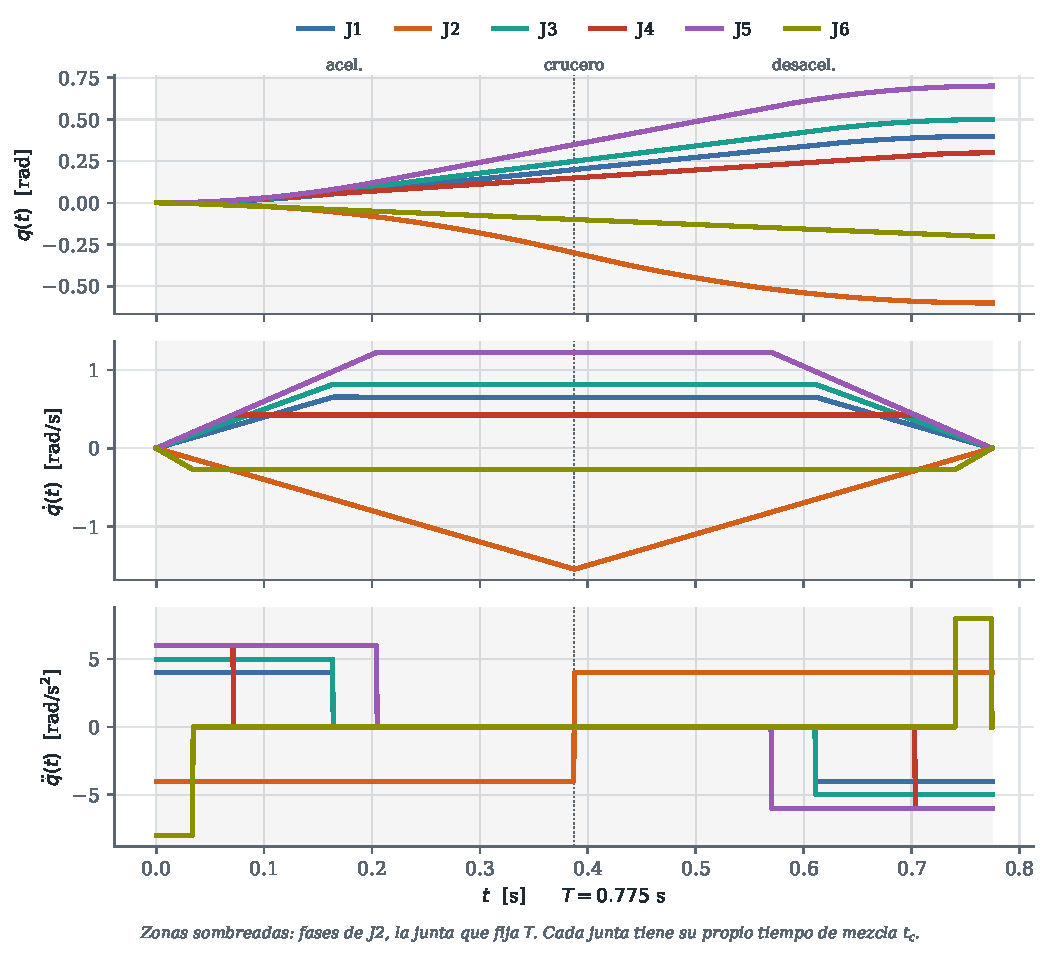
\includegraphics[width=\columnwidth]{fig_lspb.pdf}}
\caption{Perfiles LSPB de posición, velocidad y aceleración. Las zonas
sombreadas marcan las fases de mezcla parabólica. Se verifica reposo en
ambos extremos.}
\label{fig:lspb}
\end{figure}

Sobre el caso de referencia de la cátedra ($q_i = 0$, $q_f = 2$~rad,
$t_f = 3$~s, $\ddot q_c = 1$~rad/s$^2$) la implementación devuelve
$t_c = 1{,}0000$~s y velocidad de crucero $1{,}0000$~rad/s. La
aceleración mínima factible según \eqref{eq:factible} resulta
$0{,}8889$~rad/s$^2$, por debajo del valor empleado, de modo que el
perfil admite tramo de crucero.

\subsection{Jacobiano}

La primera columna derivada a mano en $\bm{q}=\bm{0}$ coincide con la
implementación en $2{,}08\times10^{-18}$. La validación cruzada por
diferencias finitas sobre la matriz completa arroja
$3{,}25\times10^{-8}$, consistente con el truncamiento esperable de un
esquema de primer orden. Dos métodos independientes que coinciden son
evidencia considerablemente más fuerte que un método que simplemente no
falla.

\subsection{Experimento de singularidad}

La Tabla~\ref{tab:sing} registra la aproximación a $q_5 = 0$.

\begin{table}[htbp]
\caption{Aproximación a la singularidad de muñeca}
\label{tab:sing}
\centering
\footnotesize
\begin{tabular}{@{}rrrr@{}}
\toprule
$q_5$ [rad] & $\sigma_{\min}$ & $\kappa(J)$ &
$\lVert\dot{\bm{q}}\rVert$ [rad/s] \\
\midrule
$10^{-1}$ & $2.680\times10^{-2}$ & $6.80\times10^{1}$ & $1.65\times10^{1}$ \\
$10^{-2}$ & $2.679\times10^{-3}$ & $6.81\times10^{2}$ & $1.65\times10^{2}$ \\
$10^{-3}$ & $2.678\times10^{-4}$ & $6.81\times10^{3}$ & $1.65\times10^{3}$ \\
$10^{-4}$ & $2.678\times10^{-5}$ & $6.81\times10^{4}$ & $1.65\times10^{4}$ \\
$10^{-5}$ & $2.678\times10^{-6}$ & $6.81\times10^{5}$ & $1.65\times10^{5}$ \\
$10^{-6}$ & $2.678\times10^{-7}$ & $6.81\times10^{6}$ & $1.65\times10^{6}$ \\
\bottomrule
\end{tabular}
\end{table}

El ajuste logarítmico da
$\lVert\dot{\bm{q}}\rVert \sim q_5^{-1.000}$, y la Fig.~\ref{fig:div}
lo muestra en escala doble logarítmica, donde una ley de potencia es
una recta cuya pendiente es el exponente.

\begin{figure}[htbp]
\centerline{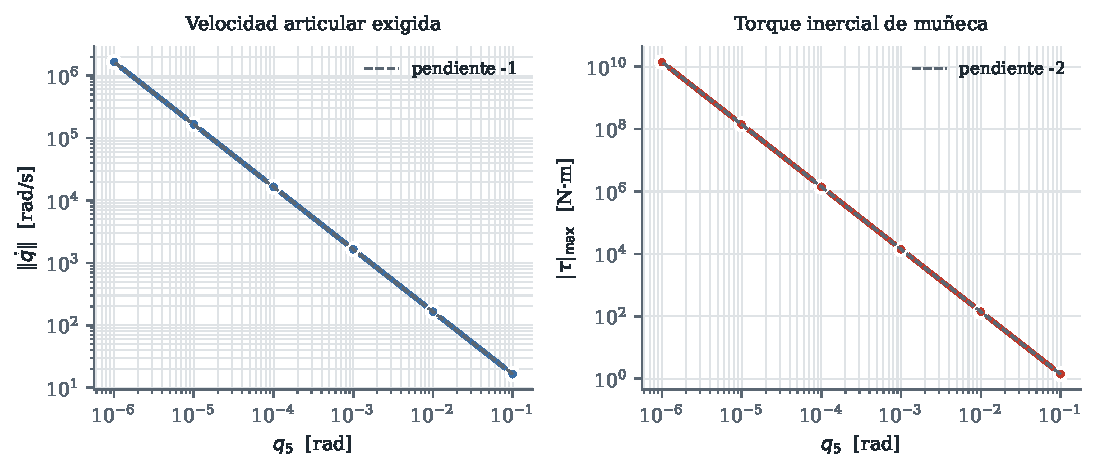
\includegraphics[width=\columnwidth]{fig_divergencia.pdf}}
\caption{Amplificación de la velocidad articular al aproximarse a la
singularidad, en escala logarítmica doble.}
\label{fig:div}
\end{figure}

Esta ley vale \textbf{para la dirección de tarea solicitada}, y la
precisión importa. Para un Jacobiano cuadrado regular las cotas
correctas son
\begin{equation}
    \frac{\lVert\dot{\bm{x}}\rVert}{\sigma_{\max}}
    \;\le\; \lVert\dot{\bm{q}}\rVert \;\le\;
    \frac{\lVert\dot{\bm{x}}\rVert}{\sigma_{\min}},
    \label{eq:cotas}
\end{equation}
de modo que $\sigma_{\min}$ acota por \emph{arriba}, no por abajo. La
descomposición
$\lVert\dot{\bm{q}}\rVert^2 = \sum_i (\bm{u}_i^{T}\dot{\bm{x}})^2/\sigma_i^2$
explica por qué: la divergencia depende de la proyección de la tarea
sobre el modo que pierde capacidad. Una tarea compatible permanece
acotada.

En la singularidad exacta, $\sigma_{\min} = 2{,}83\times10^{-18}$ y el
rango cae de 6 a 5. Las cinco direcciones restantes permanecen
accesibles, tres de ellas con valores singulares superiores a la
unidad. El robot no se detiene: pierde un grado de libertad
instantáneo de seis.

Conviene declarar además qué devuelve la pseudoinversa en ese punto.
Ante una tarea \emph{incompatible} con la imagen de $J$, el método de
mínimos cuadrados entrega una velocidad finita pero con residuo
$\lVert J\dot{\bm{q}} - \dot{\bm{x}}\rVert = 0{,}442$: esa es la parte
de la tarea que se abandona. Ante una tarea compatible el residuo es
exactamente cero. Una velocidad finita en una singularidad no significa
que la tarea se haya cumplido.

La Fig.~\ref{fig:manip} muestra la manipulabilidad a lo largo de la
trayectoria del proyecto y contiene un hallazgo: $w = 0$ exactamente en
$t = 0$. La postura de reposo del robot es $\bm{q} = \bm{0}$, que
incluye $q_5 = 0$; es decir, la configuración de origen del IRB~120
\emph{es} la singularidad de muñeca estudiada.

\begin{figure}[htbp]
\centerline{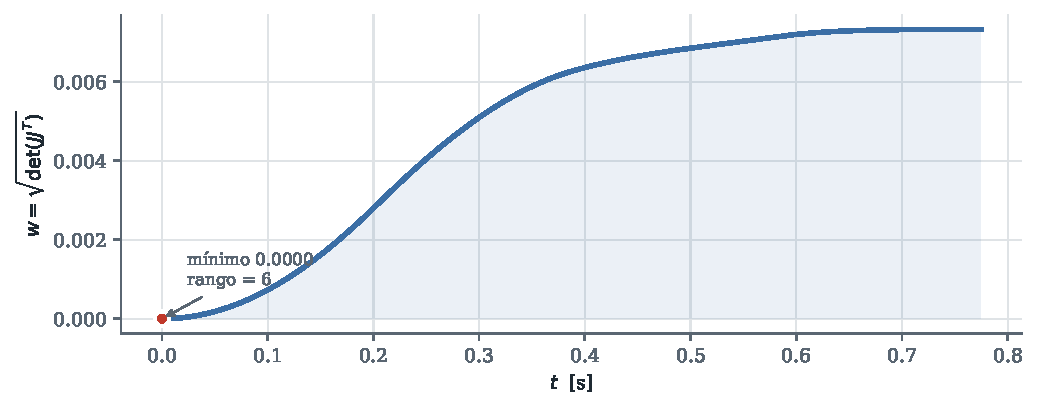
\includegraphics[width=\columnwidth]{fig_manipulabilidad.pdf}}
\caption{Manipulabilidad de Yoshikawa a lo largo de la trayectoria. El
mínimo en $t = 0$ corresponde a la postura de reposo, que es singular.}
\label{fig:manip}
\end{figure}

\subsection{Torque sobre la trayectoria}

La Tabla~\ref{tab:1r} contrasta \eqref{eq:tau1r} contra el desarrollo
analítico de referencia publicado por la cátedra \cite{b6}.

\begin{table}[htbp]
\caption{Modelo 1R en $t = 2{,}5$~s frente a la referencia}
\label{tab:1r}
\centering
\footnotesize
\begin{tabular}{@{}lrr@{}}
\toprule
\textbf{Magnitud} & \textbf{Referencia} & \textbf{Implementación} \\
\midrule
$q$ [rad]                            & $1.875$  & $1.8750$ \\
$\dot{q}$ [rad/s]                    & $0.5$    & $0.5000$ \\
$\ddot{q}$ [rad/s$^2$]               & $-1$     & $-1.0000$ \\
$\tau_{\text{inercial}}$ [N$\cdot$m] & $-0.250$ & $-0.2500$ \\
$\tau_{\text{gravedad}}$ [N$\cdot$m] & $4.679$  & $4.6798$ \\
$\tau_{\text{total}}$ [N$\cdot$m]    & $4.429$  & $4.4298$ \\
\bottomrule
\end{tabular}
\end{table}

La Fig.~\ref{fig:tau1r} presenta la serie completa con las tres
magnitudes alineadas en el tiempo.

\begin{figure}[htbp]
\centerline{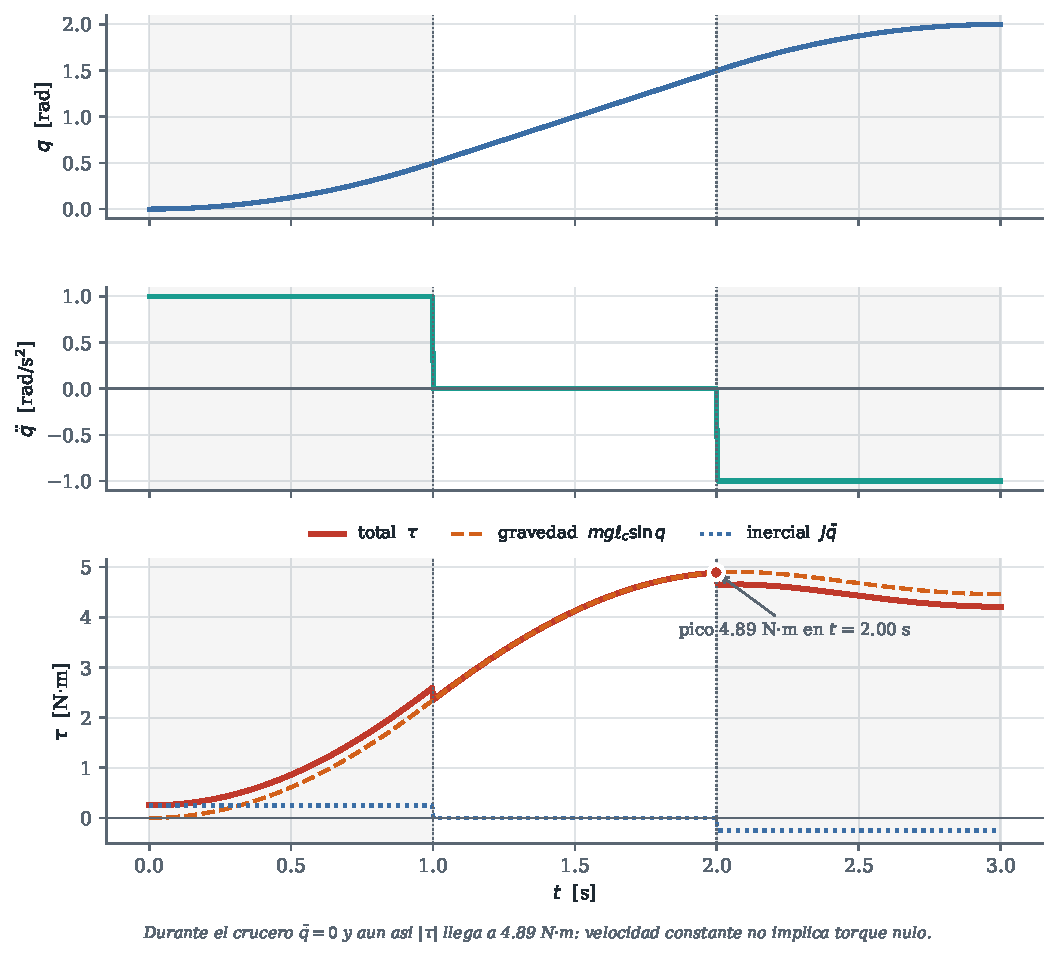
\includegraphics[width=\columnwidth]{fig_torque_1r.pdf}}
\caption{Modelo 1R: posición, aceleración y torque alineados. Durante
el crucero la aceleración es nula y el torque no lo es.}
\label{fig:tau1r}
\end{figure}

% =====================================================================
\section{Discusión}
\label{sec:discusion}

\subsection{Velocidad constante no implica torque nulo}

Durante la fase de crucero, entre $t = 1{,}002$~s y $t = 1{,}998$~s, la
aceleración es exactamente cero y el término inercial de
\eqref{eq:tau1r} se anula. Sin embargo el torque recorre el intervalo
de $2{,}36$ a $4{,}89$~N$\cdot$m. La razón es que el término
gravitatorio $mg\ell_c\sin q$ no depende de derivada alguna de $q$,
sino de la postura: mientras el eslabón esté fuera de la vertical, el
motor debe sostener su peso aunque no lo esté acelerando.

De hecho el pico de torque, $4{,}89$~N$\cdot$m, ocurre en
$t = 1{,}998$~s, con aceleración exactamente nula. Dimensionar un motor
guiándose solo por la aceleración máxima subestimaría groseramente la
demanda real.

Esta comparación exige una precaución metodológica que conviene hacer
explícita. En un perfil LSPB la aceleración alcanza su magnitud máxima
a lo largo de un \emph{intervalo} completo, no en un instante aislado.
Comparar el índice de $\arg\max|\tau|$ contra el de $\arg\max|\ddot q|$
puede por tanto producir un falso ``no coinciden''. La comparación
correcta se hace sobre valores, no sobre índices, y el resultado
depende de la trayectoria: en la del proyecto el pico sí cae en
aceleración máxima, porque su junta~2 tiene perfil triangular y carece
de tramo de crucero.

\subsection{Singularidad cinemática no es torque alto}

Las dos nociones se confunden con facilidad y conviene separarlas.

Una singularidad es una propiedad de la \emph{cinemática diferencial}:
el Jacobiano pierde rango y el manipulador pierde direcciones de
movimiento instantáneo. Es una degradación geométrica y existe con
independencia de las masas: un robot sin peso, en gravedad cero, tiene
exactamente las mismas singularidades.

Un torque alto es una propiedad de la \emph{dinámica}: expresa cuánto
esfuerzo exige una trayectoria dadas las inercias y la gravedad.

Que sean independientes se comprueba en ambos sentidos. El modelo 1R de
la Sección~\ref{sec:result} no posee singularidad alguna --- su
Jacobiano es un escalar que nunca se anula --- y aun así demanda
$4{,}89$~N$\cdot$m. Y la singularidad de muñeca del IRB~120 se alcanza
en posturas que no exigen torque gravitatorio particularmente elevado.

Donde sí existe un vínculo es indirecto, y conviene enunciarlo con
cuidado. Si se exige mantener una velocidad de tarea fija con
componente en la dirección que se pierde, la cinemática diferencial
inversa amplifica la velocidad articular; la aceleración, siendo su
derivada, hereda esa amplificación, y recién entonces el término
inercial crece. La singularidad no produce torque: produce velocidad
articular ilimitada. La distinción importa porque la mitigación es
distinta --- replanificar la trayectoria frente a redimensionar el
actuador.

\subsection{Consecuencia práctica de la singularidad en el origen}

Que la postura de reposo sea singular tiene una consecuencia que debe
enunciarse con precisión. \emph{No} es cierto que el robot no pueda
moverse bajo control cartesiano desde el reposo: puede ejecutar
cualquier tarea compatible con la imagen de $J$, que en $q_5 = 0$ sigue
teniendo dimensión 5. Lo que no puede es seguir una velocidad con
componente en la dirección perdida; intentarlo produce el residuo de
$0{,}442$ documentado antes.

Que el perfil LSPB atraviese esa configuración sin inconveniente no es
una contradicción: LSPB interpola en el espacio articular y nunca
invierte $J$.

\subsection{Sobre la interpretación de la dirección perdida}

El vector singular izquierdo asociado al valor singular nulo tiene
norma parcial $0{,}897$ en sus tres primeras componentes y $0{,}442$ en
las tres últimas. Es tentador concluir de ahí qué clase de movimiento
se pierde, pero esa comparación mezcla m/s con rad/s: para hacerla
habría que declarar una longitud característica o una métrica de tarea.

Lo que sí es incondicional, y no depende de unidades, es la caída de
rango de 6 a 5: se pierde una dirección del twist combinado. Esa es la
afirmación que el trabajo sostiene.

\subsection{Limitaciones}

Cuatro, declaradas explícitamente.

La singularidad de hombro se verificó solo por tendencia: la
manipulabilidad cae de $10^{-2}$ a $1{,}73\times10^{-4}$ al
aproximarse, pero el punto exacto no se evaluó por quedar fuera del
espacio alcanzable con orientación válida. En las familias singulares
exactas, además, el conjunto de soluciones deja de ser un conjunto
discreto de ocho ramas y pasa a contener familias continuas: en
$q_5 = 0$ se conserva $q_4 + q_6$, y con el centro de muñeca sobre el
eje de la base el ángulo $q_1$ queda indeterminado. El tratamiento
completo de esas familias queda fuera del alcance de este trabajo.

Los parámetros dinámicos son pedagógicos y no corresponden a los del
IRB~120 real, que el fabricante no publica. Las conclusiones sobre la
\emph{forma} de $\tau(t)$ son válidas; las magnitudes absolutas no
deben leerse como especificación.

El modelo dinámico ignora fricción y flexibilidad de transmisión, ambas
relevantes en un accionamiento real.

Finalmente, las validaciones de este trabajo verifican consistencia
interna, acuerdo entre métodos independientes y reproducción de
resultados publicados. No constituyen una identificación dinámica del
robot ni garantizan cobertura exhaustiva del espacio de trabajo.

% =====================================================================
\section{Conclusiones}

Se construyó y validó un pipeline completo que transita desde una pose
cartesiana objetivo hasta la demanda de torque del actuador sobre el
ABB~IRB~120.

La cinemática inversa analítica por Pieper resuelve las ocho ramas con
error del orden del épsilon de máquina. El punto de mayor contenido
ingenieril de ese bloque no fue la derivación sino el filtrado: la
distinción entre solución matemática y configuración ejecutable, que
exigió extracción numéricamente estable de los ángulos de muñeca,
tolerancia de redondeo en los topes y expansión de los representantes
articulares equivalentes. Las pruebas dirigidas que expusieron esos
tres fallos no habían sido detectadas por 2000 ensayos aleatorios, lo
que constituye en sí una conclusión metodológica: el muestreo uniforme
no visita las fronteras.

El Jacobiano geométrico, validado por dos métodos independientes,
permitió caracterizar la singularidad de muñeca no solo detectándola
sino identificando qué dirección se pierde, cuáles permanecen y qué
parte de la tarea abandona la pseudoinversa.

La evaluación del modelo 1R sobre la trayectoria LSPB cerró el ciclo
reproduciendo exactamente el resultado analítico de referencia, con la
correspondencia angular derivada y verificada en vez de supuesta.

Las dos conclusiones no triviales son que el torque no sigue al perfil
de aceleración cuando la gravedad domina, y que singularidad cinemática
y demanda dinámica son fenómenos independientes, vinculados solo de
forma indirecta a través de la cinemática diferencial inversa. Ambas
tienen consecuencia práctica directa sobre el dimensionamiento de
actuadores y sobre la planificación de trayectorias.

\begin{thebibliography}{00}
\bibitem{b1} B. Siciliano, L. Sciavicco, L. Villani y G. Oriolo,
\textit{Robotics: Modelling, Planning and Control}. Londres: Springer,
2009.
\bibitem{b2} J. J. Craig, \textit{Introduction to Robotics: Mechanics
and Control}, 4.ª ed. Upper Saddle River, NJ: Pearson, 2018.
\bibitem{b3} D. L. Pieper, ``The kinematics of manipulators under
computer control,'' tesis doctoral, Dept.\ Comput.\ Sci., Universidad
de Stanford, Stanford, CA, 1968.
\bibitem{b4} T. Yoshikawa, ``Manipulability of robotic mechanisms,''
\textit{Int.\ J. Robot.\ Res.}, vol.~4, n.º~2, pp.~3--9, 1985.
\bibitem{b5} ABB Robotics, \textit{Product Specification IRB 120},
doc.\ 3HAC035960-001. Västerås, Suecia: ABB AB, 2023.
\bibitem{b6} B. Quiroga Turdera, ``Guía oficial y rúbrica de
evaluación: Hito 2,'' IMT-342 Robótica, Universidad Católica Boliviana
``San Pablo'', Sede Tarija, 2026.
\bibitem{b7} Grupo VEVAS, ``Proyecto Final Integrador --- ABB IRB 120,''
repositorio de código, 2026. [En línea]. Disponible en:
\url{https://github.com/FlorenciaFrigerio/pfi-vevas-irb120}
\end{thebibliography}

\end{document}
